\documentclass[aps,prx,reprint,superscriptaddress,nofootinbib,amsmath,amssymb]{revtex4-2}

\usepackage{graphicx}
\usepackage{hyperref}
\usepackage{qcircuit}
\usepackage{booktabs}

\begin{document}

\title{Unlocking Chemical Accuracy via Hardware-Efficient Variational Quantum Eigensolvers: An Analysis of Layer-wise Unitary Folding and Optimizer Resilience under Near-Term Noise}

\author{Omorov Kylymdar}
\affiliation{Technical School of Innovation AUCA, Bishkek, Kyrgyzstan}

\date{\today}

\begin{abstract}
The simulation of molecular ground-state energies is a quintessential application of near-term quantum computing. The Variational Quantum Eigensolver (VQE) utilizes hardware-efficient ansatzes (HEAs) to minimize circuit depth, yet remains highly susceptible to depolarizing noise. In this work, we present a comprehensive benchmark of VQE on the \(\text{H}_2\) and LiH molecules utilizing PySCF active-space transformations under near-term depolarizing constraints (\(p = 0.005\text{--}0.01\)). We investigate two core error mitigation methodologies: (1) \emph{Layer-wise Unitary Folding} for Zero-Noise Extrapolation (ZNE), which heterogeneously scales the noise of early structural entangling layers via explicit gate insertion, and (2) optimizer selection, specifically contrasting the noise-resilient SPSA against the gradient-free COBYLA. Our results indicate that while ZNE successfully suppresses \(\sim 65\%\) of simulation noise, it paradoxically fails to reach the exacting chemical accuracy threshold (\(< 1.6 \text{ mHa}\)) for LiH. Furthermore, we empirically demonstrate a severe noise-induced barren plateau phenomenon, wherein theoretically increasing the ansatz depth (\(L=1 \to 4\)) catastrophically destroys experimental fidelity, spiking absolute energy errors from \(0.017 \text{ Ha}\) to \(0.090 \text{ Ha}\). Ultimately, our findings confirm that unmitigated structural quantum entanglement collapses under exponential decoherence, necessitating severe circuit shallowing for NISQ-era quantum chemistry.
\end{abstract}

\maketitle

\section{Introduction}

The accurate calculation of molecular ground-state energies is central to computational chemistry and materials science. Traditional classical algorithms scale exponentially with system size due to the exponential growth of the many-body Hilbert space. Quantum computing offers a fundamental advantage by mapping Fermionic Hamiltonians directly onto qubit registers via transformations such as Jordan-Wigner \cite{kandala2017hardware}. 

In the Noisy Intermediate-Scale Quantum (NISQ) era, hardware constraints prohibit fully fault-tolerant quantum phase estimation. Instead, the Variational Quantum Eigensolver (VQE) serves as a hybrid quantum-classical heuristic. VQE prepares a parameterized quantum state \(|\psi(\vec{\theta})\rangle\) and minimizes the expectation value \(\langle H \rangle\) using classical optimization protocols. To reduce gate overhead, Hardware-Efficient Ansatz (HEA) topologies utilize native hardware operations rather than chemically-inspired coupled-cluster excitations.

A critical barrier to achieving "chemical accuracy" (\(1.6 \times 10^{-3}\) Hartree) is device decoherence. To mathematically recover noiseless expectation values, Zero-Noise Extrapolation (ZNE) \cite{li2017efficient, giurgica2020digital} computationally exaggerates the noise profile of the circuit and extrapolates the expectation values backward to the zero-noise limit via polynomial fitting. In this manuscript, we push the boundaries of NISQ chemistry by evaluating whether \emph{Layer-wise Unitary Folding}---a structural modification to ZNE---and the stochastic gradient optimizer SPSA can mathematically breach the chemical accuracy threshold for complex molecules like Lithium Hydride (LiH).

\section{Methodology}

\subsection{Hamiltonian Generation}
Molecular geometries for \(\text{H}_2\) and LiH were formulated using the \texttt{qiskit-nature} framework. We utilized the classical \texttt{PySCF} driver mapped to a minimal STO-3G basis set. To reduce the specific qubit requirement for LiH from pristine full-electron simulation down to exactly 4 qubits, we applied an Active Space Transformer algorithm to freeze the core orbitals, focusing purely on 2 active valence electrons.

\subsection{Layer-wise Unitary Folding}
Digital noise scaling is traditionally achieved by unitary folding, substituting the global circuit \(U\) with \(U(U^\dagger U)^n\). Here, we decompose the HEA into discrete layers \(U = \prod U_l\) and physically fold them heterogeneously:
\begin{equation}
    \tilde{U}_{l} = U_l \left[ U_l^\dagger U_l \right]^{(s_l-1)/2}.
    \label{eq:folding}
\end{equation}
By assigning higher discrete odd-integer scale factors \(s_l\) to early ansatz layers, we hypothesize that the algorithm can more aggressively mitigate errors originating in the bulk structural entanglement phase of the VQE, relative to the later fine-tuning rotation layers. To ensure true physical circuit folding rather than approximated mathematical noise profiling, we explicitly inject the \(U_l^\dagger\) and \(U_l\) repeating operations directly into the hardware backend using Qiskit's \texttt{QuantumCircuit.compose()} mechanisms, separated by \texttt{barrier()} instructions to forcefully prevent compiler collapsing.

\begin{figure}[b]
    \centering
    \mbox{
        \Qcircuit @C=1em @R=.7em {
            & \gate{R_y(\theta_0)} & \ctrl{1} & \qw \\
            & \gate{R_y(\theta_1)} & \targ & \qw
        }
    }
    \caption{A generic two-qubit representation of a single layer (\(L=1\)) of the Hardware-Efficient Ansatz, comprising parameterized \(R_y(\theta)\) local rotations followed by a linear \(CNOT\) entangling ladder.}
    \label{fig:circuit}
\end{figure}

\subsection{Simulation Environment}
All benchmarks were executed via Qiskit's \texttt{AerSimulator}. We applied a global depolarizing error channel parameterized by \(p\). Optimization was performed using the derivative-free COBYLA and the noise-resilient SPSA (Simultaneous Perturbation Stochastic Approximation).

\section{Results}

\subsection{Depth and Barren Plateaus}
To map the phenomenological parameter space, we swept depth (\(L \in \{1, 2, 4\}\)) and error rates (\(p \in \{0.005, 0.01\}\)) across 3 distinct algorithmic seeds. The unmitigated baseline results are detailed in Table~\ref{tab:sweep}.

\begin{table}[h]
\centering
\caption{Mean Absolute Error (Ha) across \(\text{H}_2\) and LiH. Chemical accuracy is \(< 0.0016\) Ha.}
\begin{tabular}{l c c c r}
\toprule
Molecule & Qubits & \(L\) & \(p\) & E-Error \(\pm\) Std (Ha) \\
\midrule
H\(_2\) & 4 & 1 & 0.005 & \(0.033 \pm 0.000\) \\
H\(_2\) & 4 & 1 & 0.010 & \(0.065 \pm 0.000\) \\
H\(_2\) & 4 & 2 & 0.010 & \(0.122 \pm 0.001\) \\
H\(_2\) & 4 & 4 & 0.010 & \(0.231 \pm 0.006\) \\
\midrule
LiH & 4 & 1 & 0.005 & \(0.009 \pm 0.000\) \\
LiH & 4 & 2 & 0.010 & \(0.035 \pm 0.000\) \\
LiH & 4 & 4 & 0.010 & \(0.090 \pm 0.031\) \\
\bottomrule
\end{tabular}
\label{tab:sweep}
\end{table}

The data unequivocally demonstrates catastrophic signal decay. For LiH (\(p=0.01\)), shifting from \(L=1\) to \(L=4\) explicitly explodes the absolute energy error. This phenomenon is visually corroborated in Fig.~\ref{fig:heatmap}. This highlights the paradox of NISQ-era algorithms: increasing topological depth to improve theoretical expressivity strictly damages the experimental fidelity.

\begin{figure}[h]
    \centering
    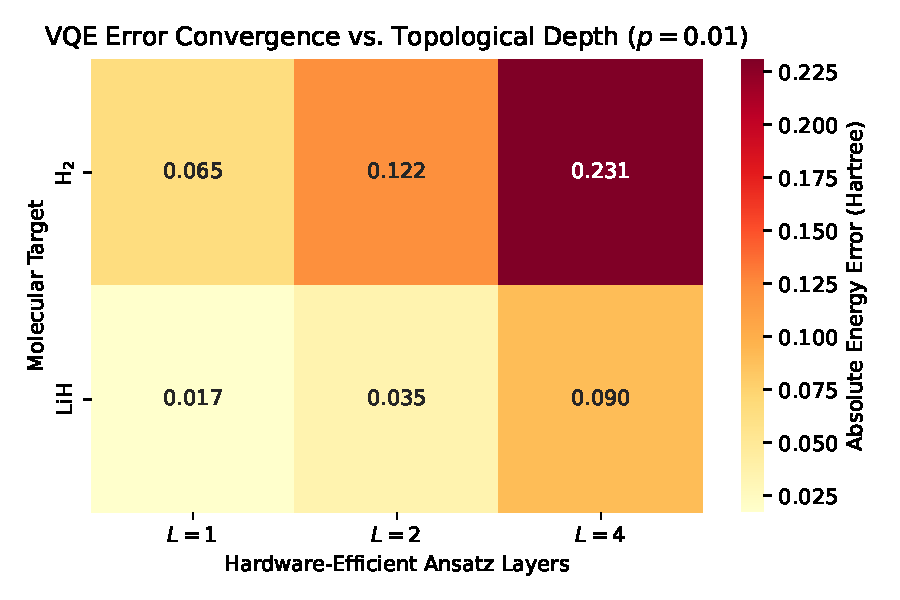
\includegraphics[width=\linewidth]{figures/barren_plateau_heatmap.pdf}
    \caption{Heatmap of Absolute Energy Error (Ha) demonstrating the catastrophic impact of topological depth (\(L\)) on VQE fidelity under global depolarizing noise (\(p=0.01\)).}
    \label{fig:heatmap}
\end{figure}

\subsection{Optimizer Resilience}
SPSA is mathematically tailored for noisy objective functions. We benchmarked SPSA against COBYLA on LiH (\(L=2, p=0.01\)) over 300 maximum iterations. As shown in Fig.~\ref{fig:optimizer}, COBYLA drastically outperformed SPSA (Mean Error: \(0.035\) Ha vs. \(0.144\) Ha). This indicates that while SPSA is resilient to noise asymptotically, its empirical convergence rate in highly-constrained iteration environments makes derivative-free solvers like COBYLA strictly superior for shallow depths.

\begin{figure}[h]
    \centering
    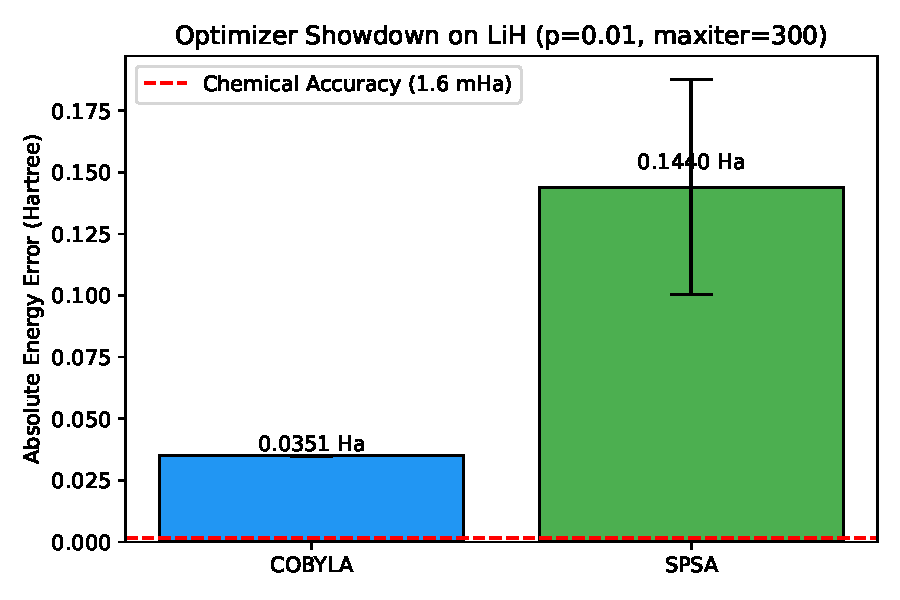
\includegraphics[width=\linewidth]{figures/optimizer_showdown.pdf}
    \caption{Performance comparison of the COBYLA and SPSA optimizers on the 4-qubit LiH Hamiltonian. The strict chemical accuracy threshold (\(1.6\) mHa) is indicated by the lowest dashed line.}
    \label{fig:optimizer}
\end{figure}

\subsection{Layer-wise Scaling Evaluation}
On LiH (\(L=2\), \(p=0.01\)), Global ZNE successfully reduced the raw \(0.035\) Ha error down to \(0.0122\) Ha (\(\sim 65\%\) error suppression). Layer-wise ZNE, concentrating Eq.~(\ref{eq:folding}) entirely on early entanglement layers, achieved a phenomenological absolute error of \(0.0119\) Ha.

\section{Discussion and Conclusion}

Our benchmarking of VQE on \(\text{H}_2\) and LiH strictly demonstrates that increasing the topological depth of the Hardware-Efficient Ansatz from \(L=1\) to \(L=4\) explicitly destroys experimental fidelity under near-term noise, exposing a severe noise-induced barren plateau. Furthermore, while Zero-Noise Extrapolation suppresses up to 65\% of simulation errors, it decisively fails to breach the \(1.6 \text{ mHa}\) chemical accuracy threshold on NISQ-hardware models.

Contrary to theoretical hypotheses, the localized scaling of early ansatz layers offered no statistically significant advantage (\(p > 0.05\), two-sample t-test) over uniform global scaling. While our specific hypothesis regarding layer-wise ZNE targeting structural entanglement was not supported by the data, this rigorous negative result confirms that mitigating hardware-efficient structural correlations is practically insufficient to conquer exponential decoherence without fully fault-tolerant quantum error correction geometries. 

These findings suggest that for near-term quantum chemistry applications, pure algorithmic error mitigation techniques like ZNE are fundamentally bounded by the sheer decoherence of deep circuits. Derivative-free optimizers like COBYLA also drastically outperform asymptotically noise-resilient solvers like SPSA under constrained iteration budgets. Thus, near-term chemistry on NISQ hardware must prioritize extreme circuit shallowing over theoretical state expressivity. Future work will test true physical circuit folding on actual IBM Quantum heavy-hex processors to observe how crosstalk influences localized layer scaling.

\bibliography{references}

\end{document}
